\chapter{Numerical Results}
\label{ch:numerical-results}

\section{QPC}
\begin{figure}[ht]
%\begin{minipage}[b]{0.49\linewidth}
\centering
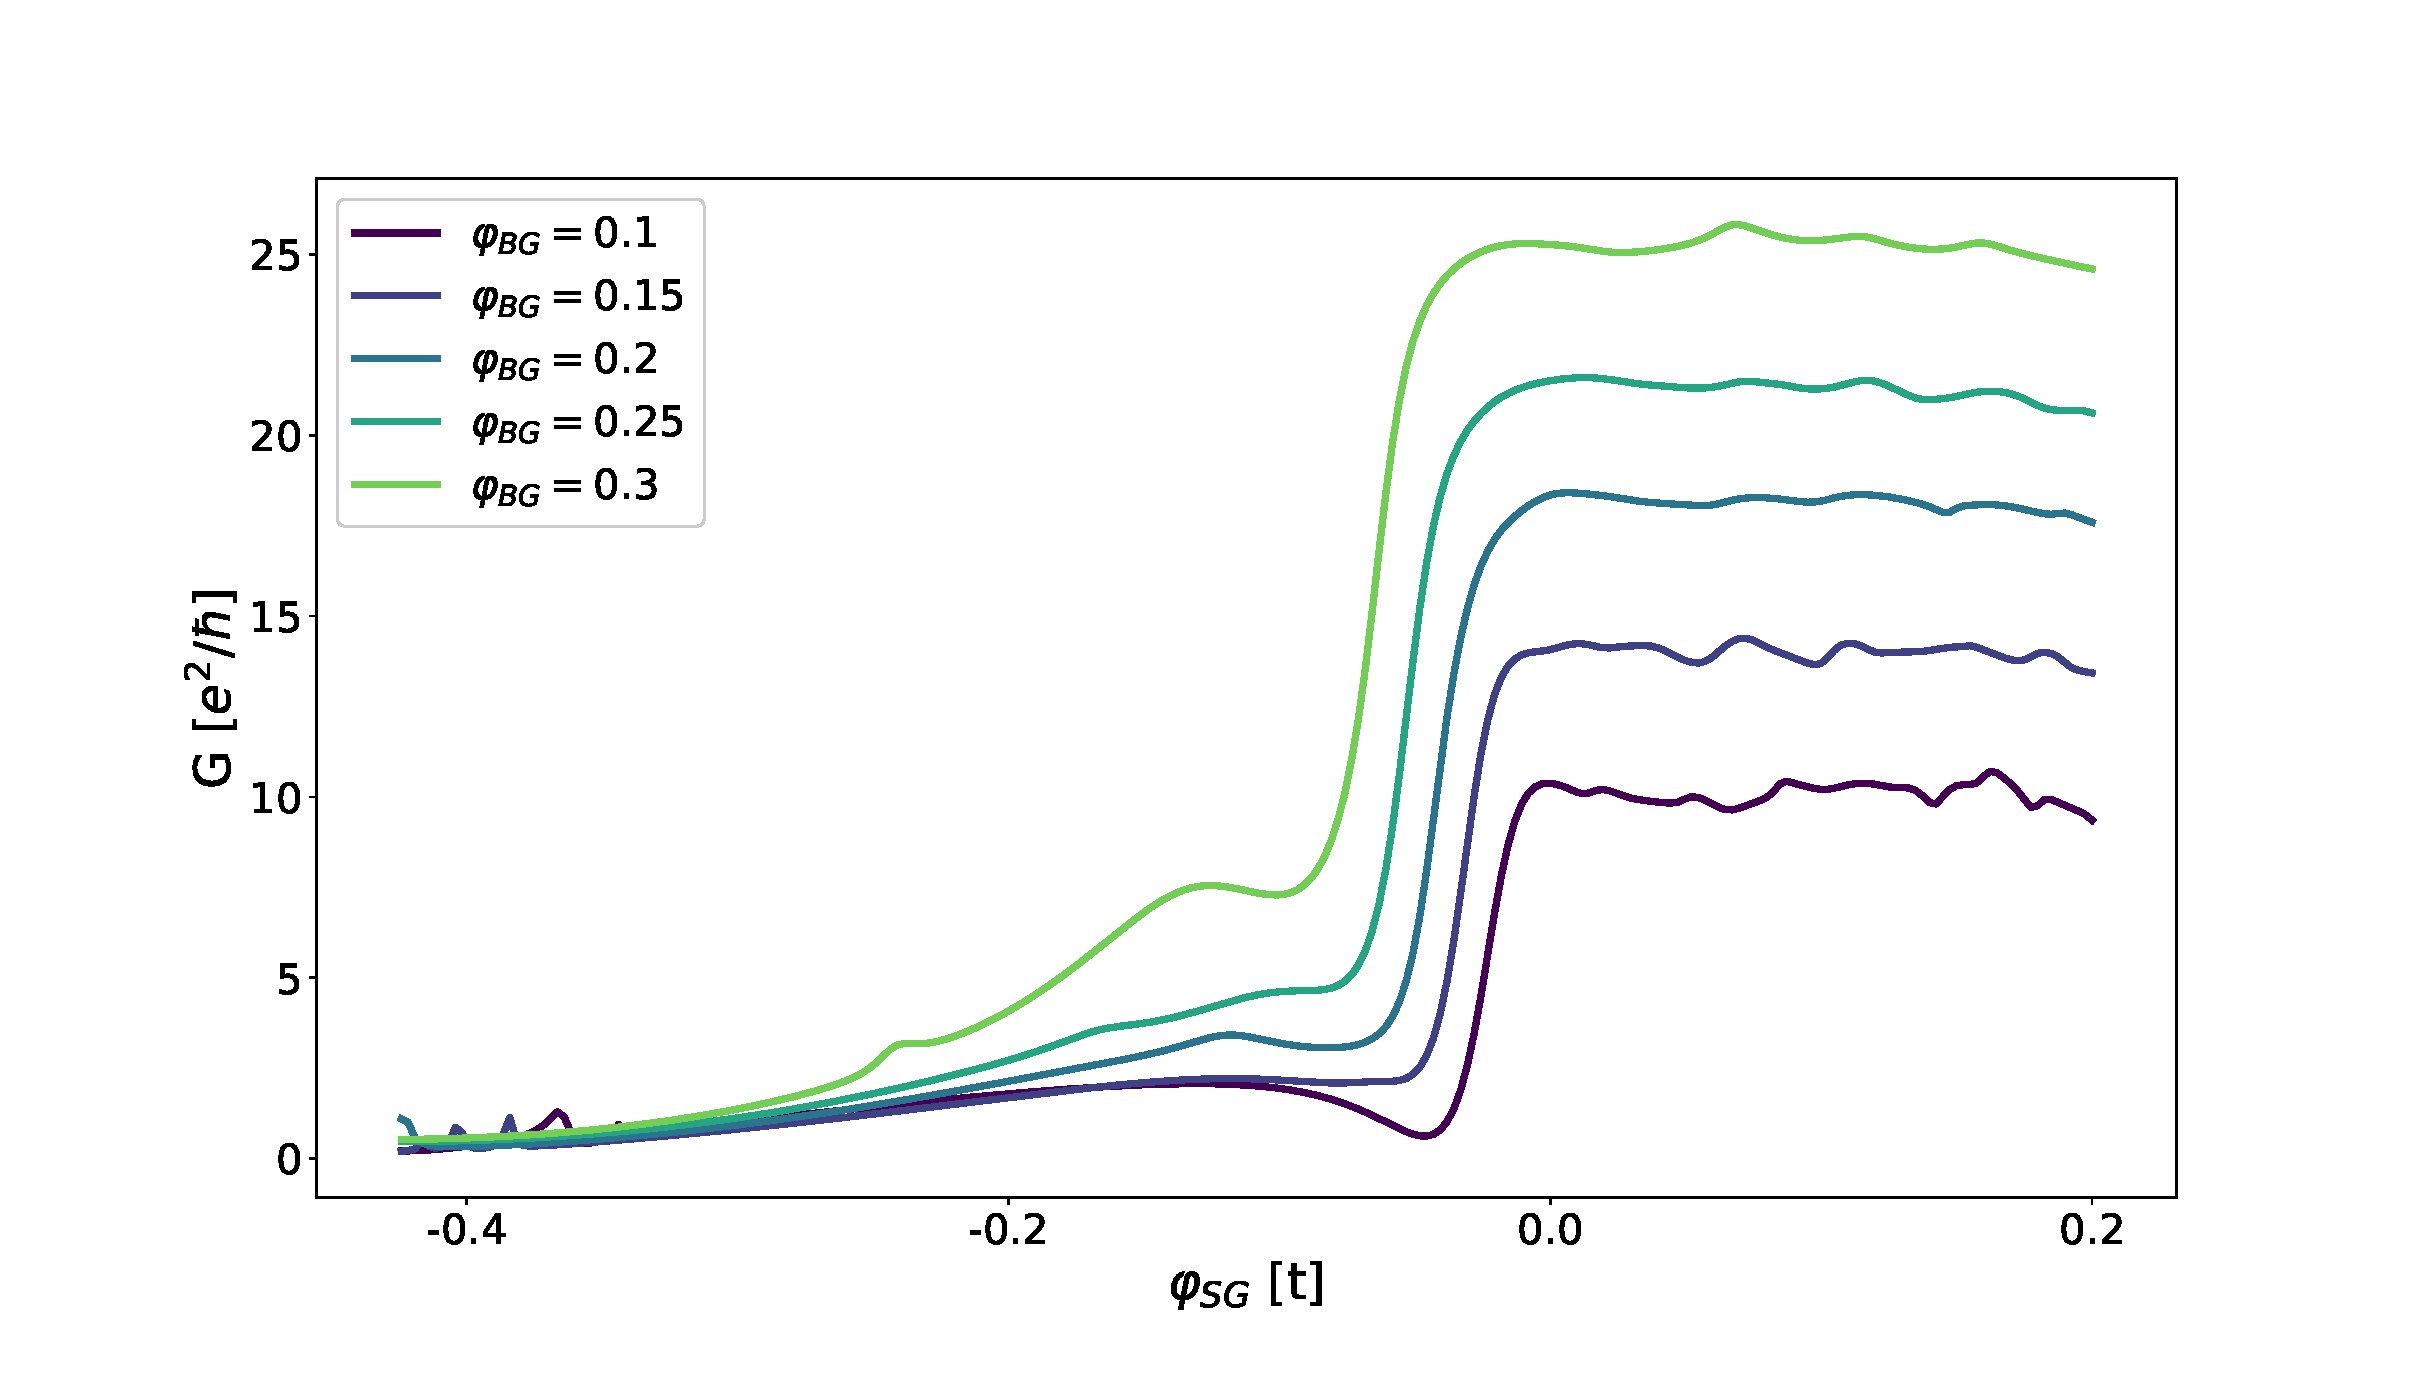
\includegraphics[width=0.8\textwidth]{figure/numericalmodel/qpc-conductance}
\caption{Conductance of the QPC system for different back-gate potentials. Even at a back-gate potential of $\varphi_{BG} = 0.3$, the overal conductance is too high to observe current confinement.} \label{fig:qpc-conductance}
%\end{minipage}
%\hspace{0.5cm}
\end{figure}
%\begin{minipage}[b]{0.49\linewidth}
\begin{figure}
\centering
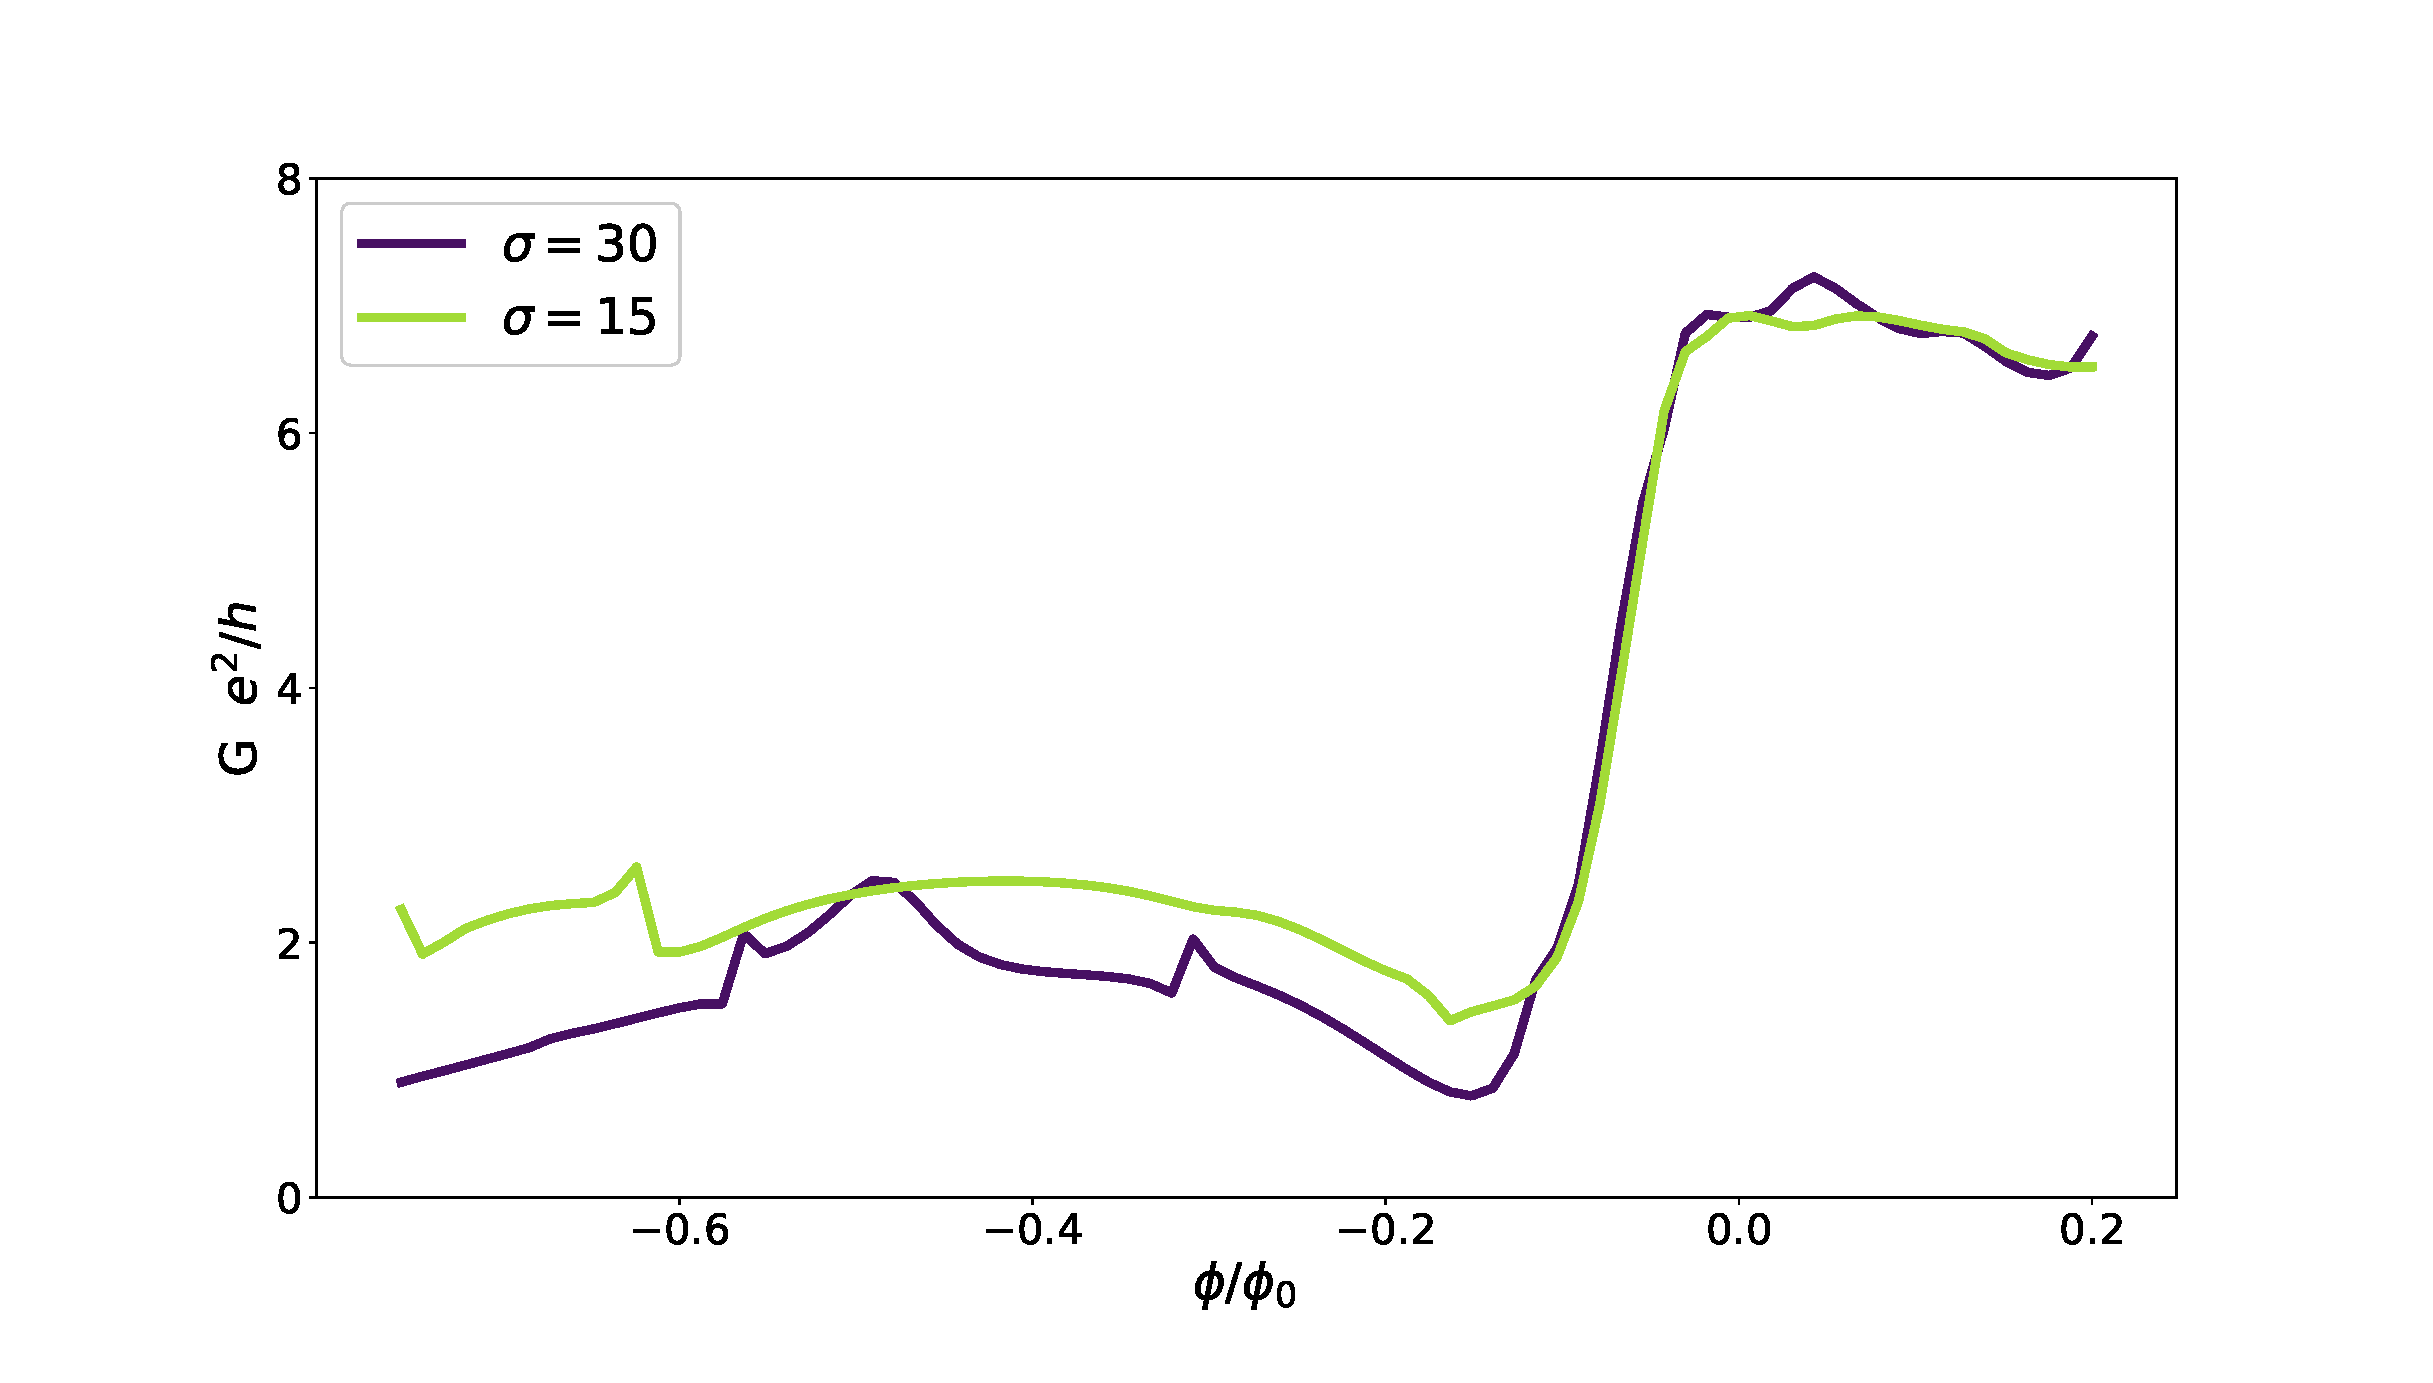
\includegraphics[width=0.8\textwidth]{figure/numericalmodel/conductance-sigma}
\caption{Conducandance of the QPC system for $\varphi_{BG} = 0.2$. The curves differ in their value of the variance of the gaussion filter, $\sigma$. For higher values of $\sigma$, the impact of the stray fields dominates and the QPC effectively becomes a reflective barrier.}\label{fig:qpc-conductance-sigma}
%\end{minipage}
\end{figure}

A fixed back-gate voltage leading to an n-doping of the scattering region is assumed, because the measurements of the experiment were conducted at fairly low charge carrier density. For increasingly negative values of the split-gate voltage, the region underneath the top gate becomes p-doped. The higher the split-gate voltage, the lower the transparency of the barrier becomes, and at a certain point, the current transport is confined to very few channels (see section \ref{sec:exp-normal-state}). In figure \ref{fig:qpc-conductance}, the conductance is plotted versus split-gate voltage. For increasingly negative values of the split-gate voltage, only few conducting channels remain. For the following calculations the back-gate voltage is chosen to be $\varphi_{BG} = 0.2$.

For increasingly positive back-gate voltage, the overall conductivity of the sample increases and the critical current cannot be confined.

The stray fields produced at the edges of the top-gate voltage are being considered as well since they are crucial for the conductive behaviour of the barrier. They are modelled as a gaussian filter applied to the vertical electric field lines:
\begin{equation}
g (x) = \frac{1}{\sqrt{2 \pi} \sigma} e^{-\frac{x^2}{2 \sigma ^2}}.
\end{equation}

Figure \ref{fig:qpc-conductance-sigma} shows two conductance lines for the same back-gate of $\varphi_{BG} = 0.2$, differing only in their $\sigma$ values. For very high values of $\sigma$, the QPC stops to function as a confinement of the current, but becomes an entirely reflective barrier. For $\sigma = 30$, the conductance falls below the threshold of 1.

\begin{figure}[h]
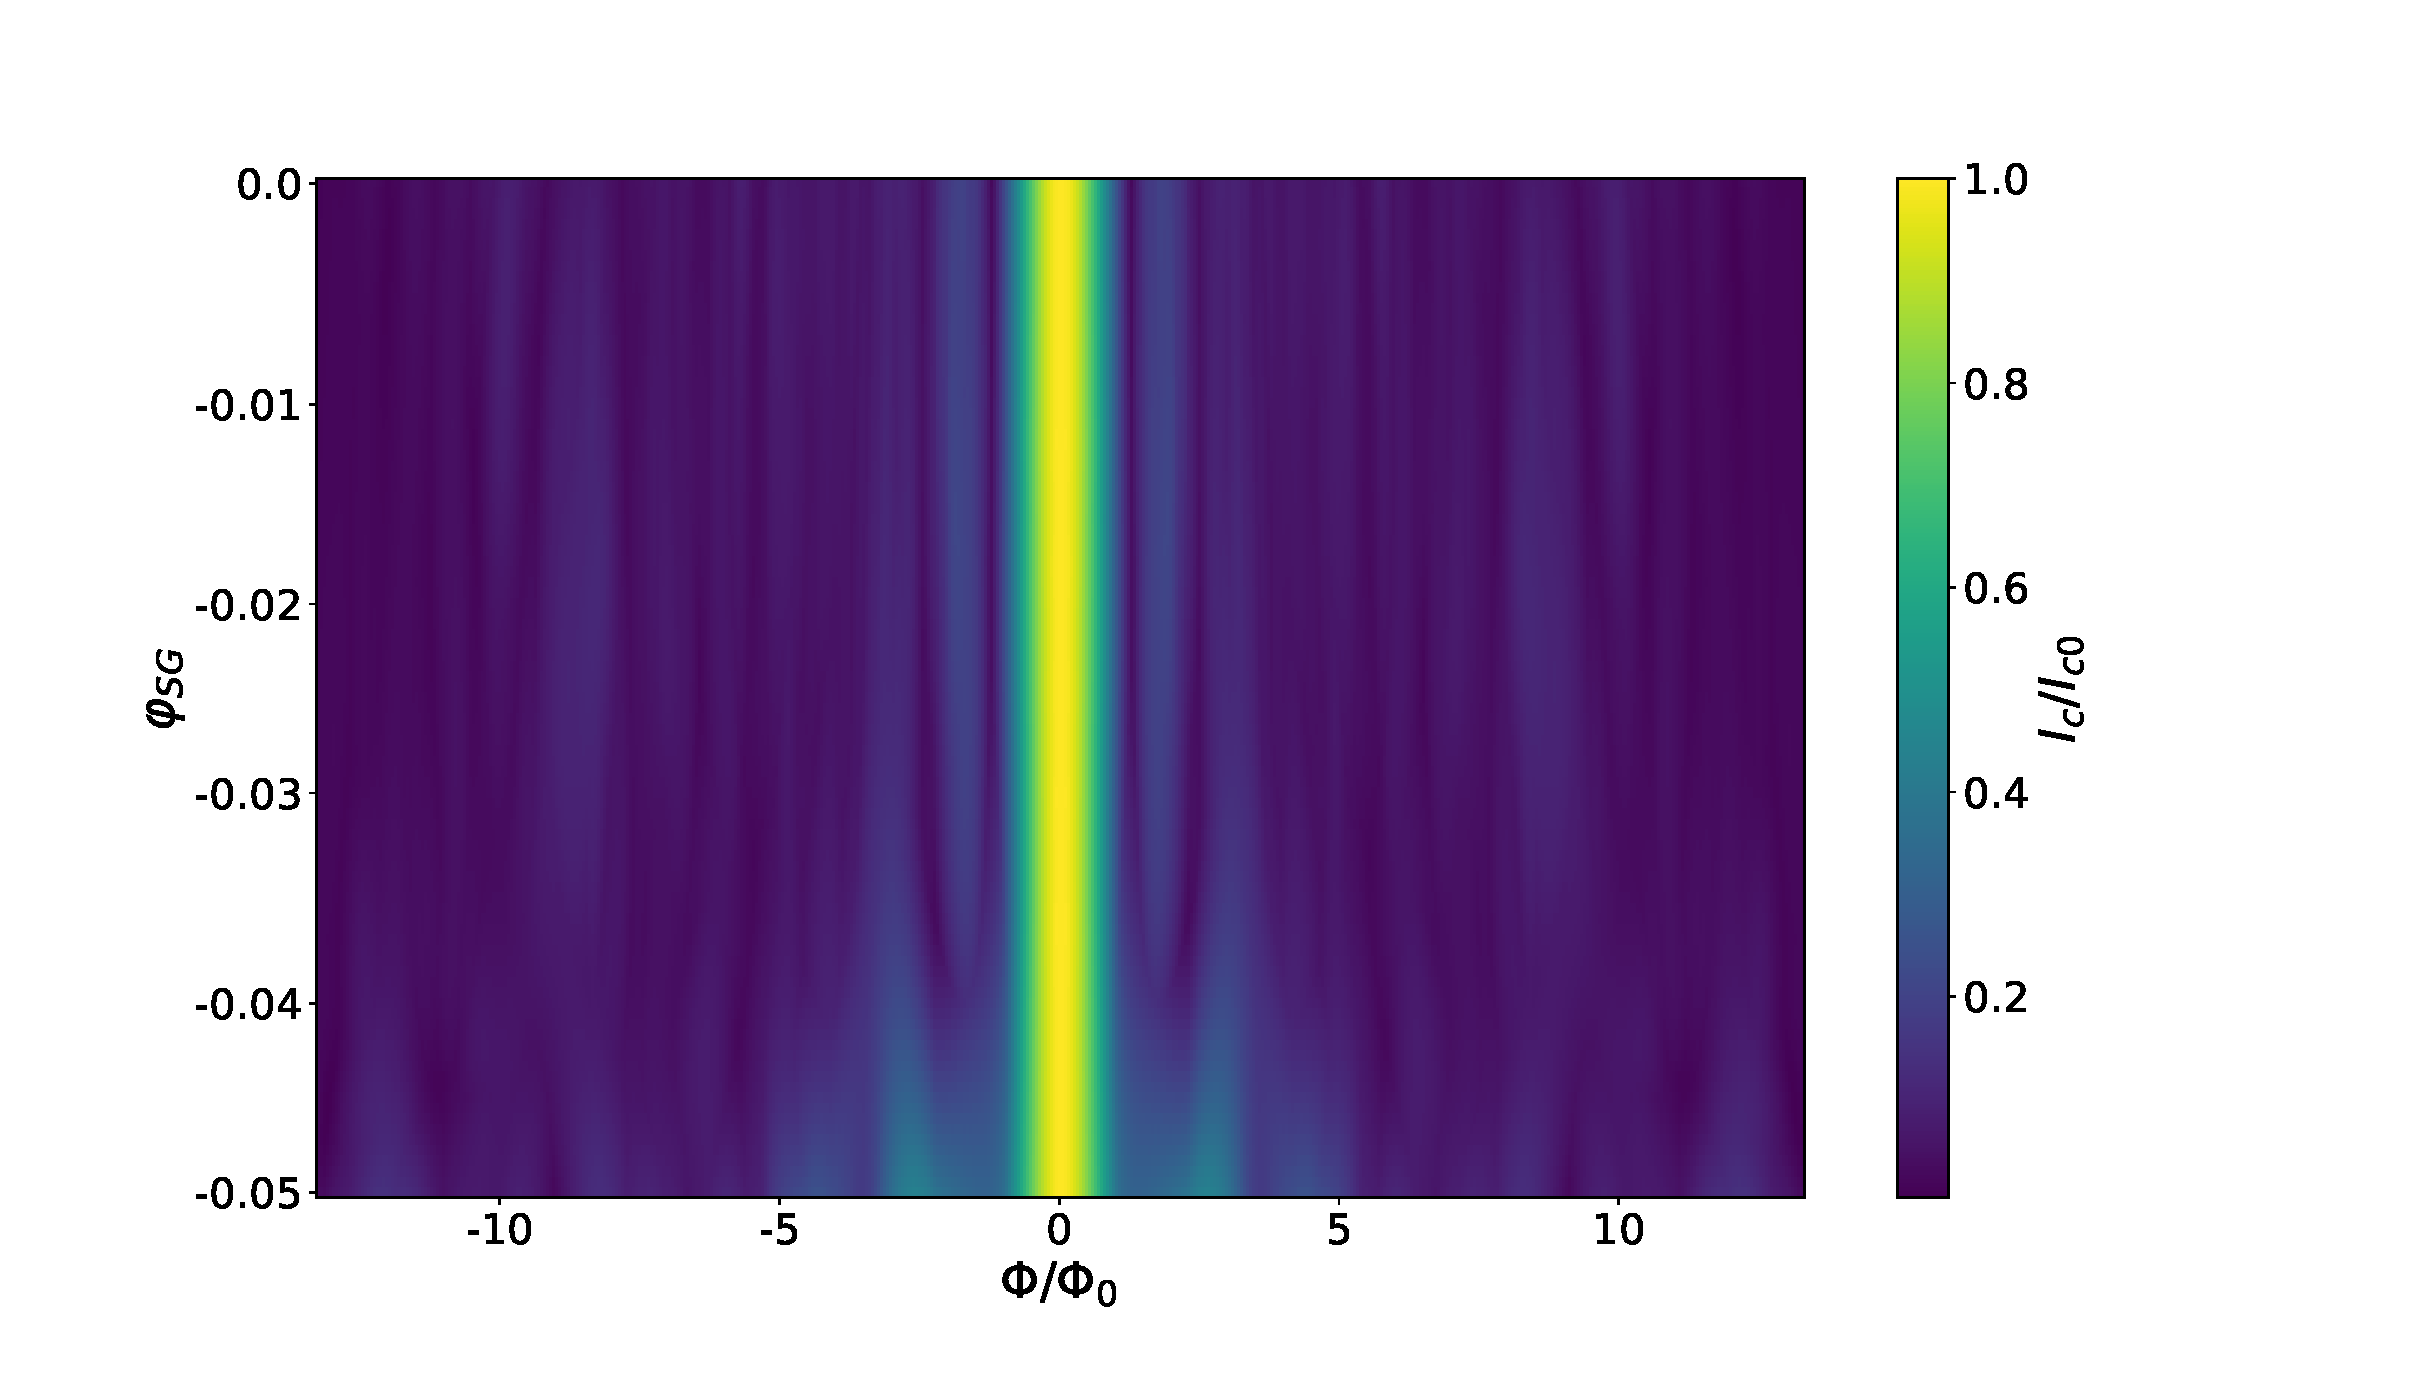
\includegraphics[width=\textwidth]{figure/numericalmodel/qpc_icnorm_heatmap}
\caption{The normalized critical current $I_c^\text{norm}$ as a function of quantised flux and split-gate potential $\varphi_{SG}$. }\label{fig:qpc-heatmap}
\end{figure}

Figure \ref{fig:qpc-heatmap} shows the the supercurrent that has been simulated by the procedure presented in \ref{sec:scattering-supercurrent}. The normalized critical current is displayed as the heat color. It is plotted against the normalized flux for different split-gate potentials. One can see clearly that for a split-gate potential of approximately 0 -- a transmissive barrier -- the critical current has the form of a Fraunhofer-like beating pattern. With increasing split-gate potential, the barrier becomes increasingly reflective, a constriction is formed, and the current is confined. A bell-shaped pattern is observed. This corresponds well to the findings presented in \ref{ch:experiment}. It should be noted that the transition from beating pattern to bell-shaped pattern happens on a narrow range of the split-gate potential.

\section{Half-Barrier}

\begin{figure}[ht]
\begin{minipage}[b]{0.49\linewidth}
\centering
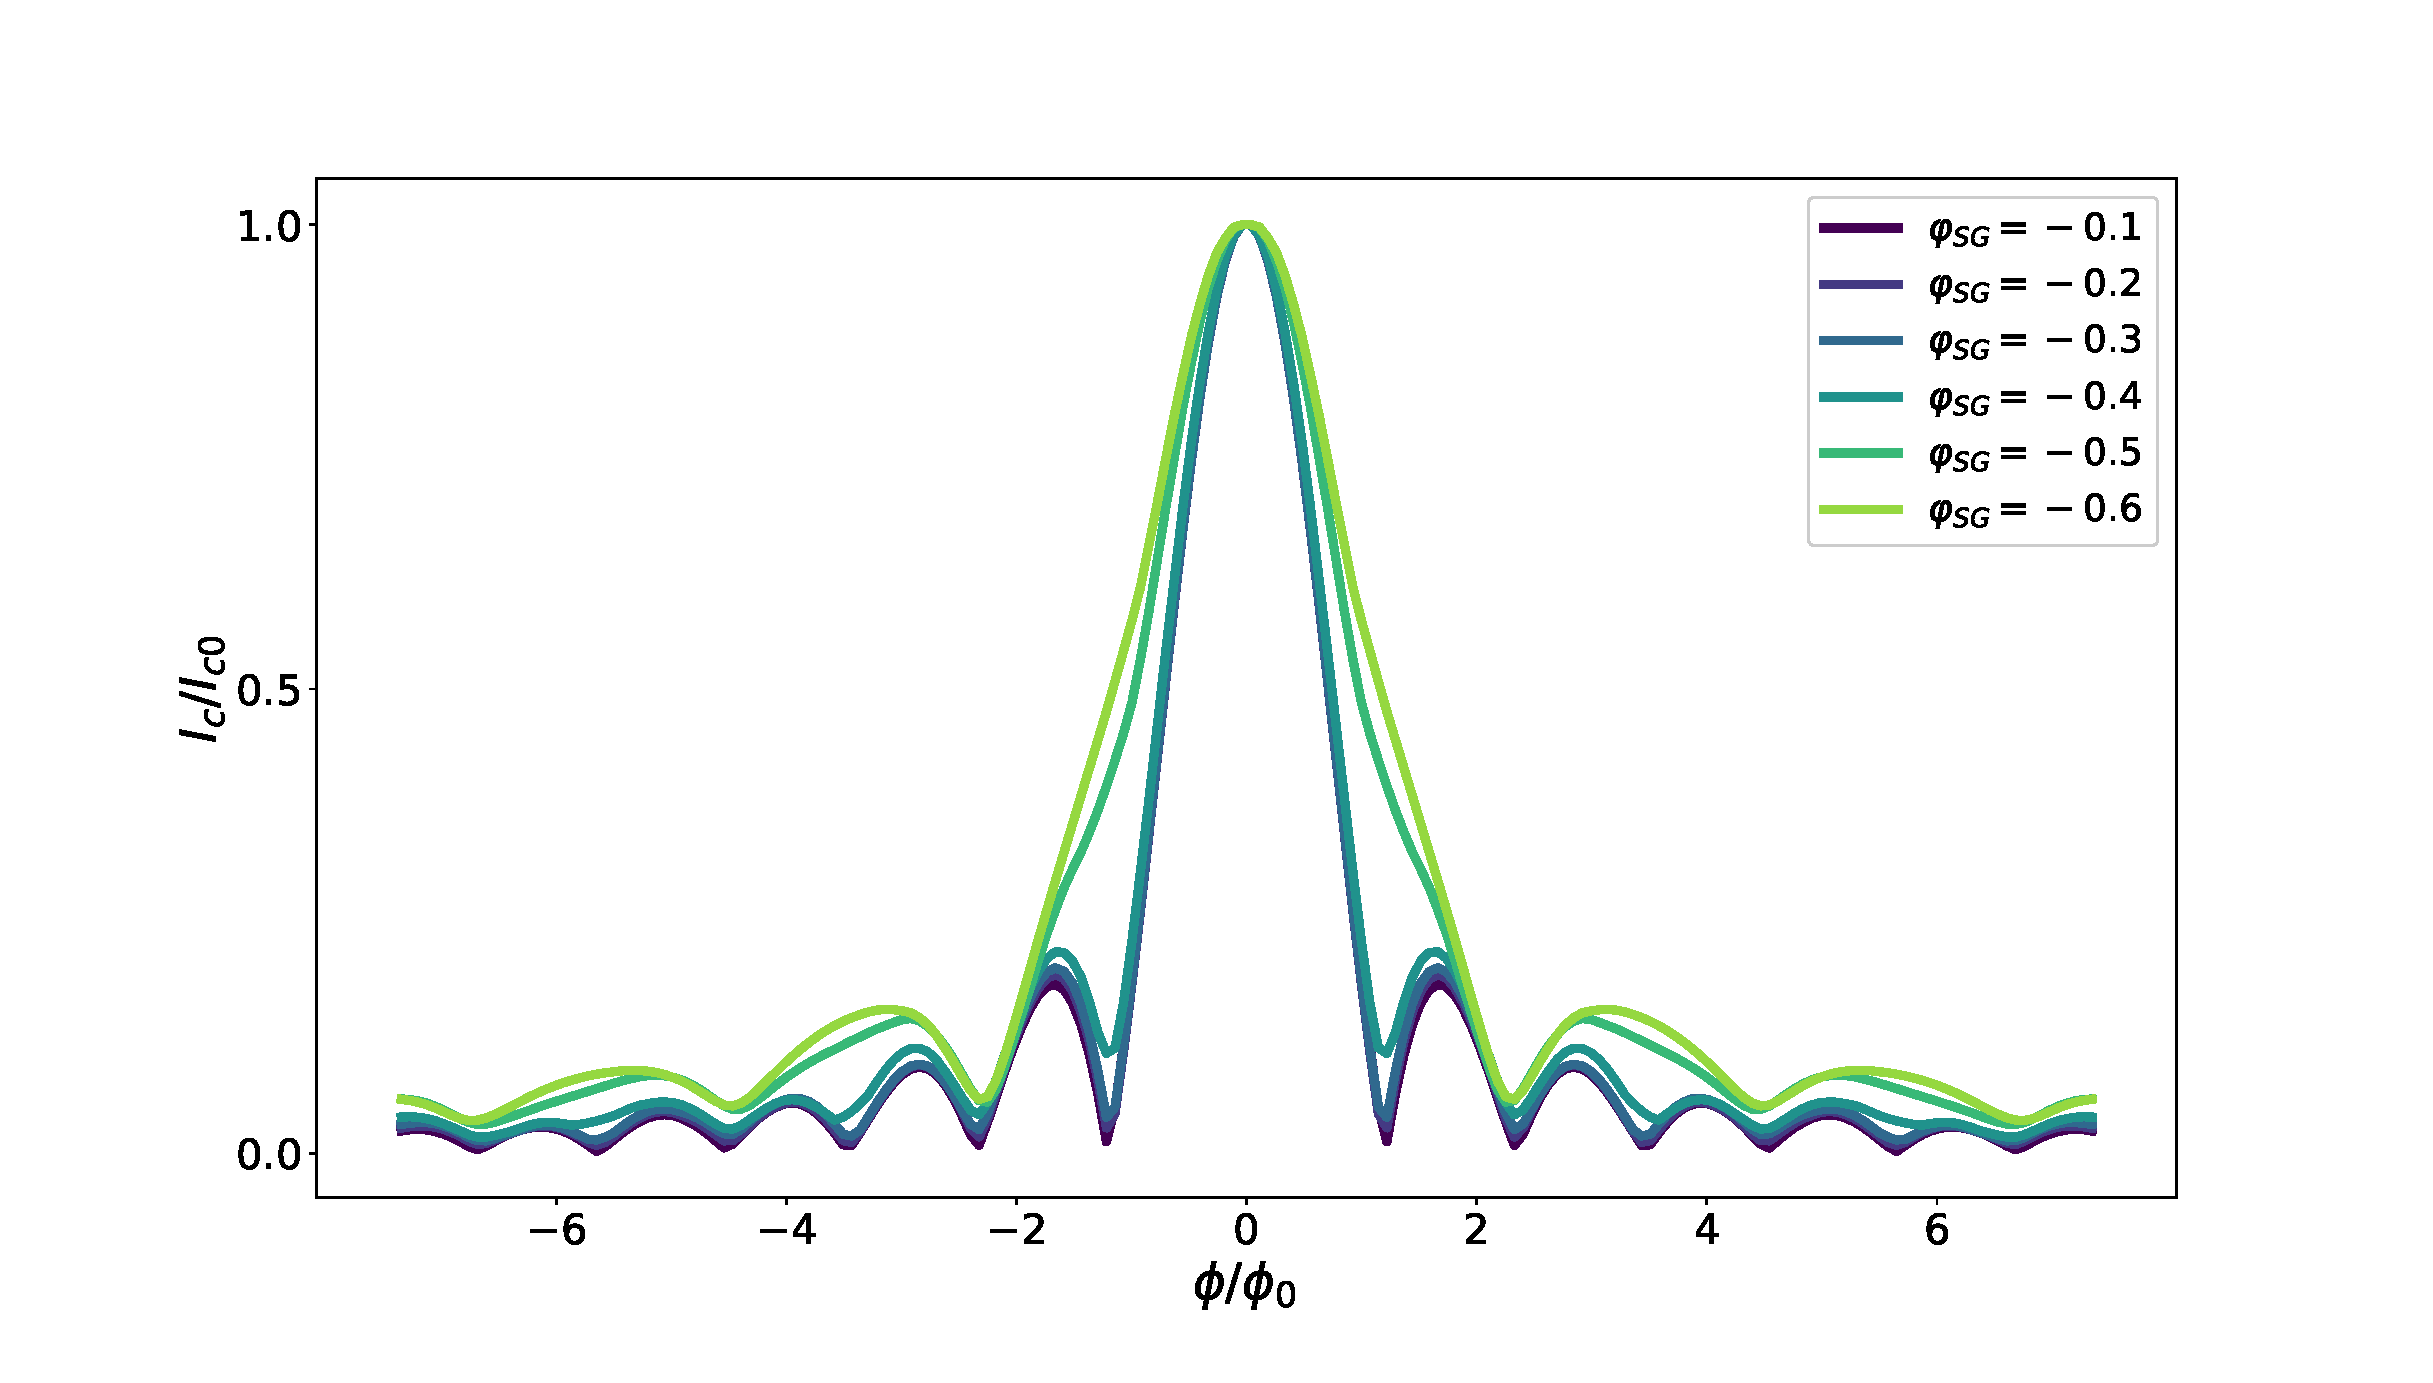
\includegraphics[width=\textwidth]{figure/numericalmodel/hb_upper}
\caption{Normalized current in the half-barrier set-up.} \label{fig:hb-norm}
\end{minipage}
%\hspace{0.5cm}
\begin{minipage}[b]{0.49\linewidth}
\centering
\includegraphics[width=\textwidth]{figure/numericalmodel/hb_upper_abs}
\caption{Absolute current in the half-barrier set-up.}\label{fig:hb-abs}
\end{minipage}
\end{figure}

The two fingers of the QPC experiment can be tuned individually, so measurements of individually gated (half-barrier) set-ups  were included in the experimental set-up. As of yet, no measurement data has been published, though.

The simulations have been carried out with a higher back-gate potential, which explains the higher values of the split-gate potential in the following plots. It is not important to have a low charge carrier density, because this set-up does not aim to confine the current. A back-gate potential of as high as $\varphi_{BG} = 0.8$ has been chosen.

The plot in figure \ref{fig:hb-abs} shows that when the barrier is fully formed, $I_{c0}$ is halved compared to its value when there is no split-gate. Figure \ref{fig:hb-norm} illustrates that as the barrier forms, the periodicity of the pattern almost doubles. This behaviour is observed in the experiment as well.

\begin{figure}[ht]
\centering
\begin{minipage}[b]{0.3\linewidth}
\centering
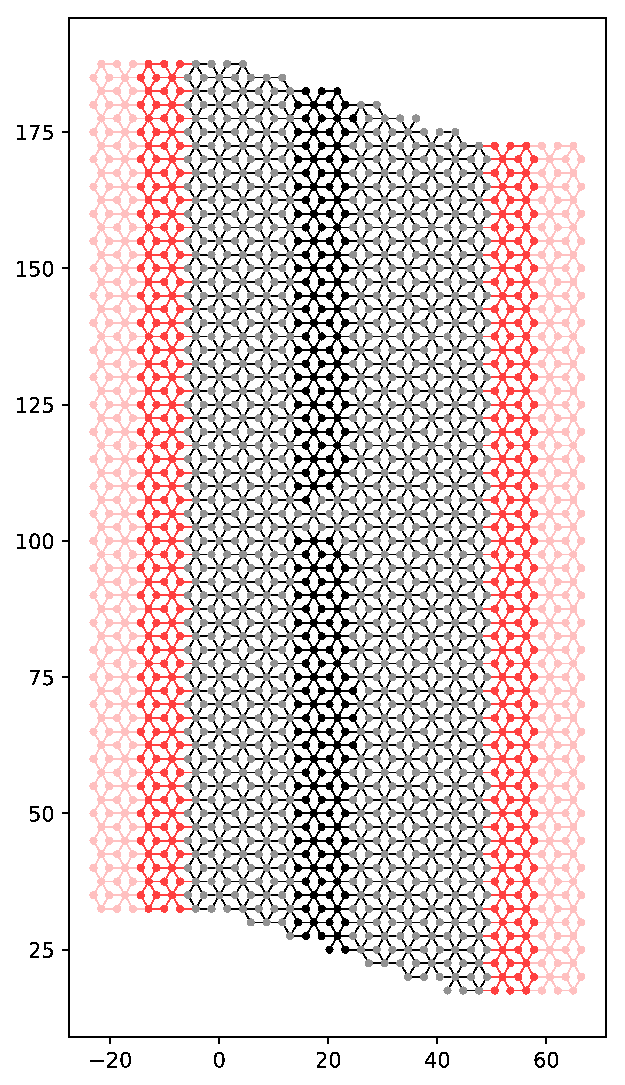
\includegraphics[width=\textwidth]{figure/numericalmodel/qpc-system}
%\caption{QPC system} \label{fig:qpc-syste}
\end{minipage}
\hspace{1.5cm}
\begin{minipage}[b]{0.3\linewidth}
\centering
\includegraphics[width=\textwidth]{figure/numericalmodel/hb-system}
%\caption{Hb system}\label{fig:hb-system}
\end{minipage}
\caption{QPC and half-barrier systems. The red areas are the superconducting leads, the grey area is the normal bi-layer graphene region, and lattice sites colored black are effectively covered by the top gate. The half-barrier set-up results when only one of the fingers of the QPC are activated. It should be noticed that the superconducting material has been modelled with the same lattice structure as the normal region, which is only approximation.}\label{fig:systems}
\end{figure}

The halving of the critical current peak can be explained within the framework of the quasi-classical theory. When a barrier is fully present, only half of the trajectories connecting the superconducting leads can pass. Figure \ref{fig:systems} pictures the implementation of the sample in \texttt{kwant}. The geometry of the asymmetric sample manifests in the Fraunhofer pattern. Because of the asymmetry, the upper finger allows for more trajectories than the lower finger. The maximum current therefore saturates at a higher threshold with the upper half-barrier.

Periodicity can be understood geometrically as well: About half of the area contributes to the magnetic phase. The phase changes accordingly, which leads to a doubling of the periodicity.

\section{Wave-guide}

\begin{figure}
\centering
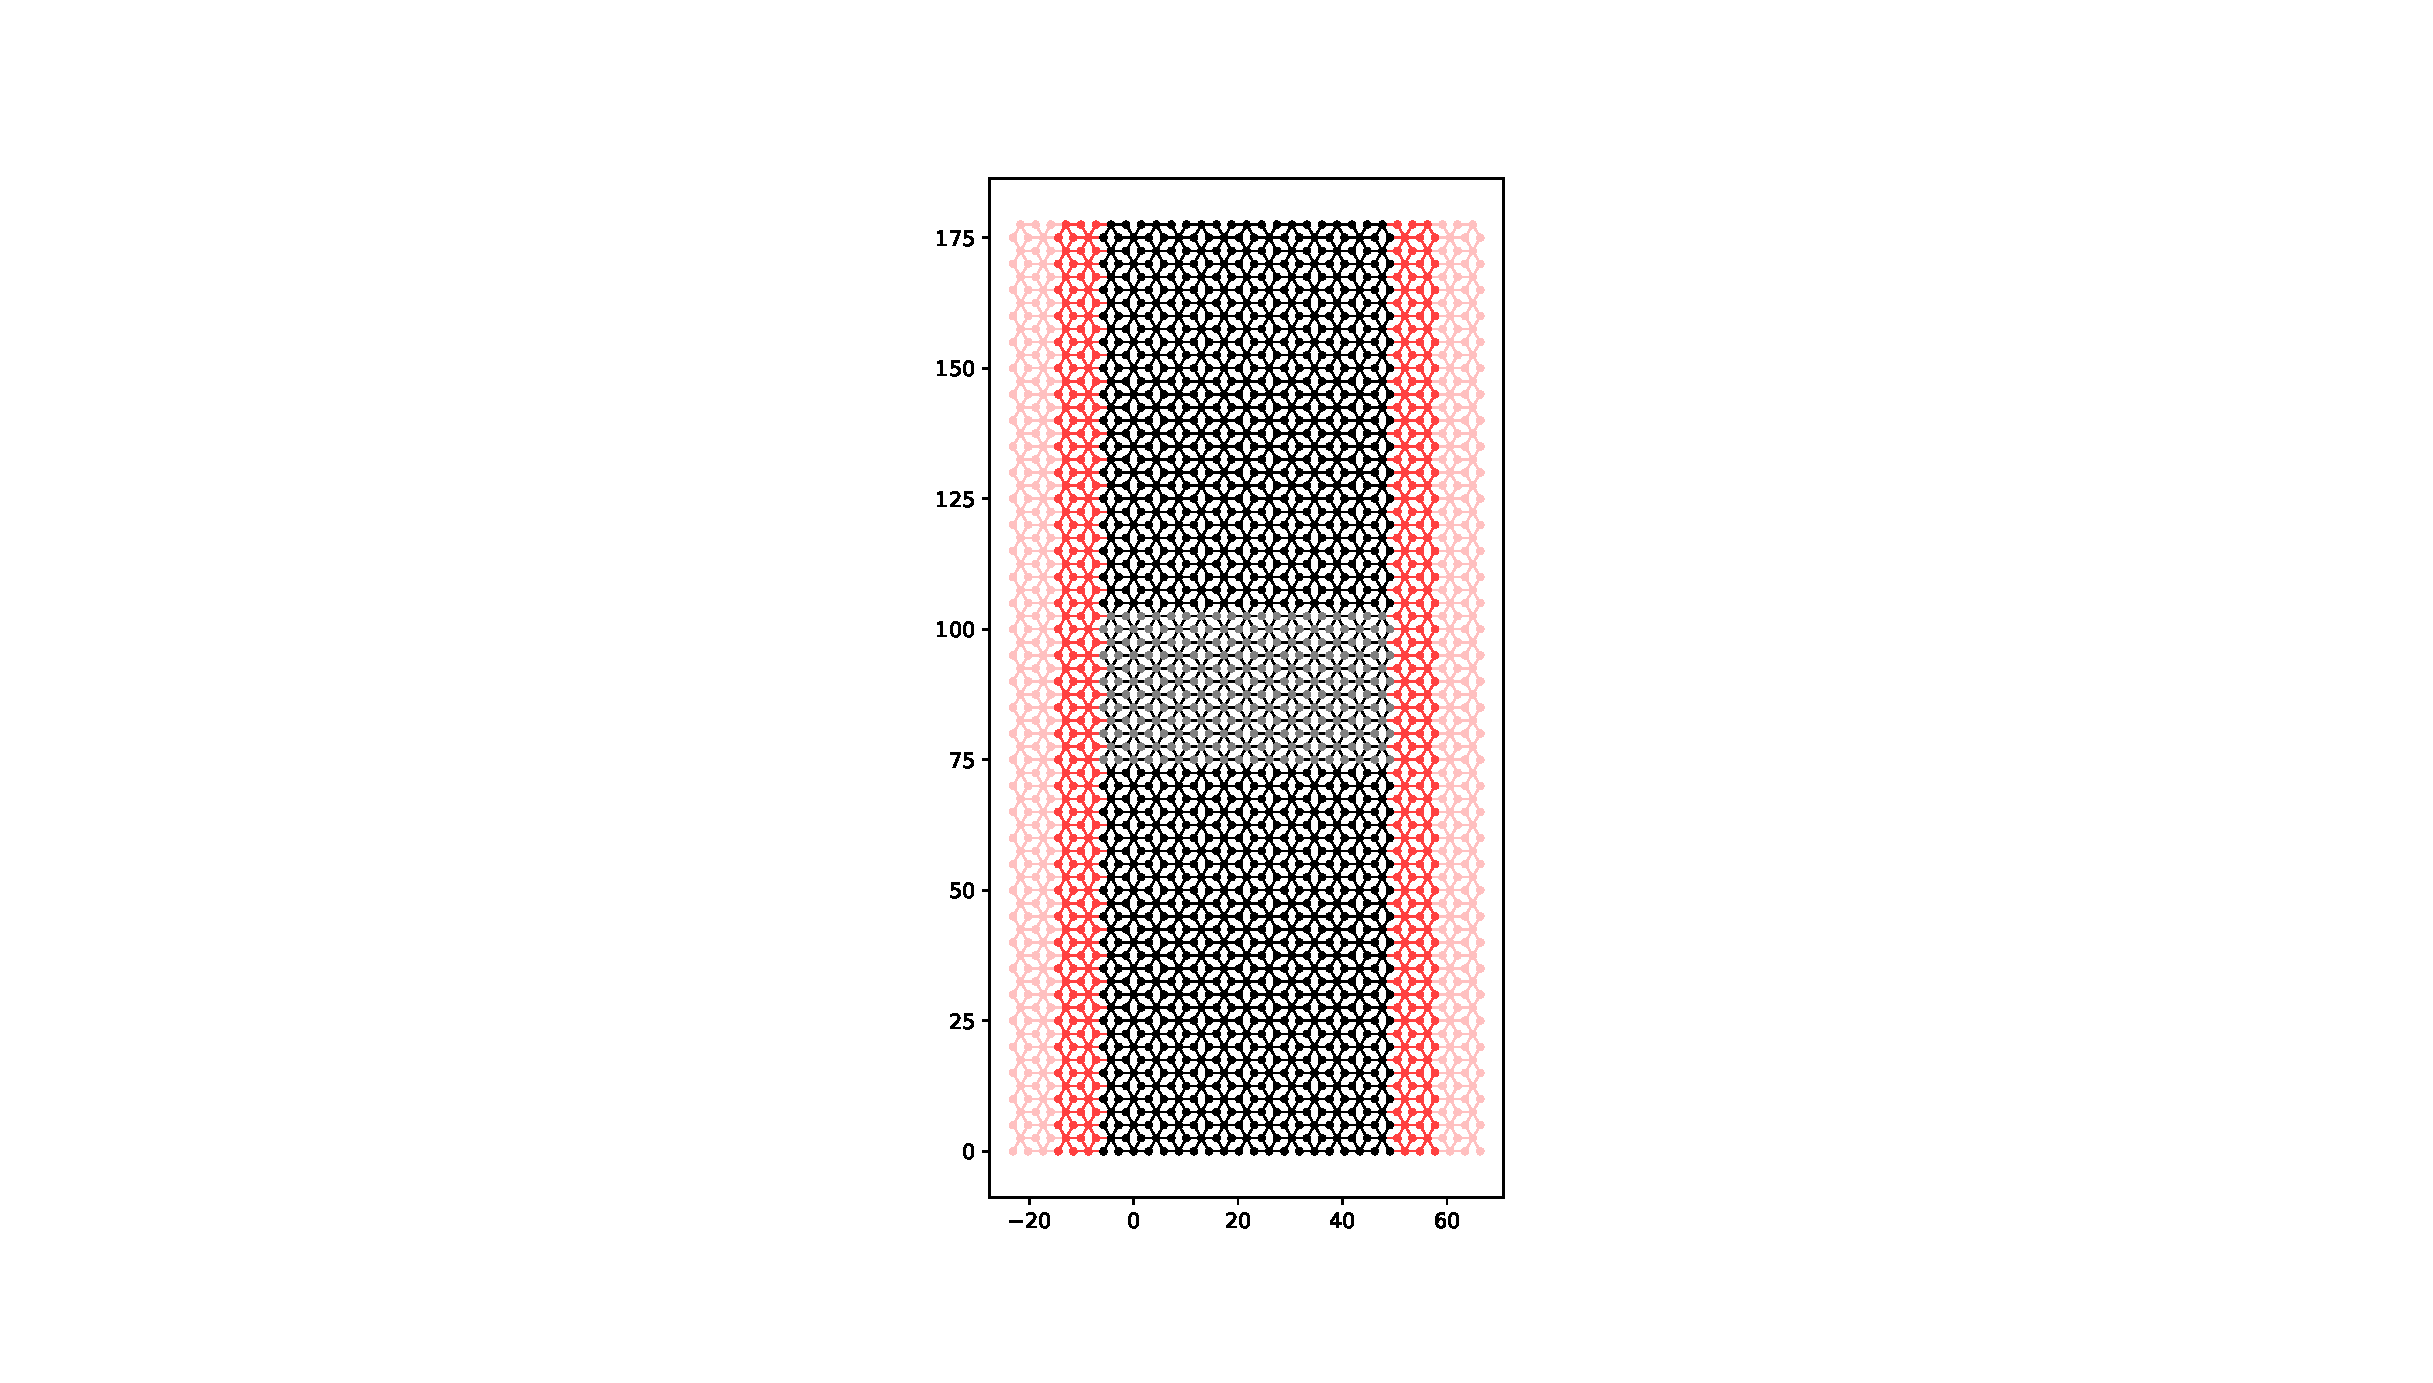
\includegraphics[width=0.8\textwidth]{figure/numericalmodel/waveguide}
\caption{Wave-guide system. The top gate covers most of the sample; only a narrow transport region remains.}\label{fig:waveguide-system}
\end{figure}

\begin{figure}[ht]
\begin{minipage}[b]{0.5\linewidth}
\centering
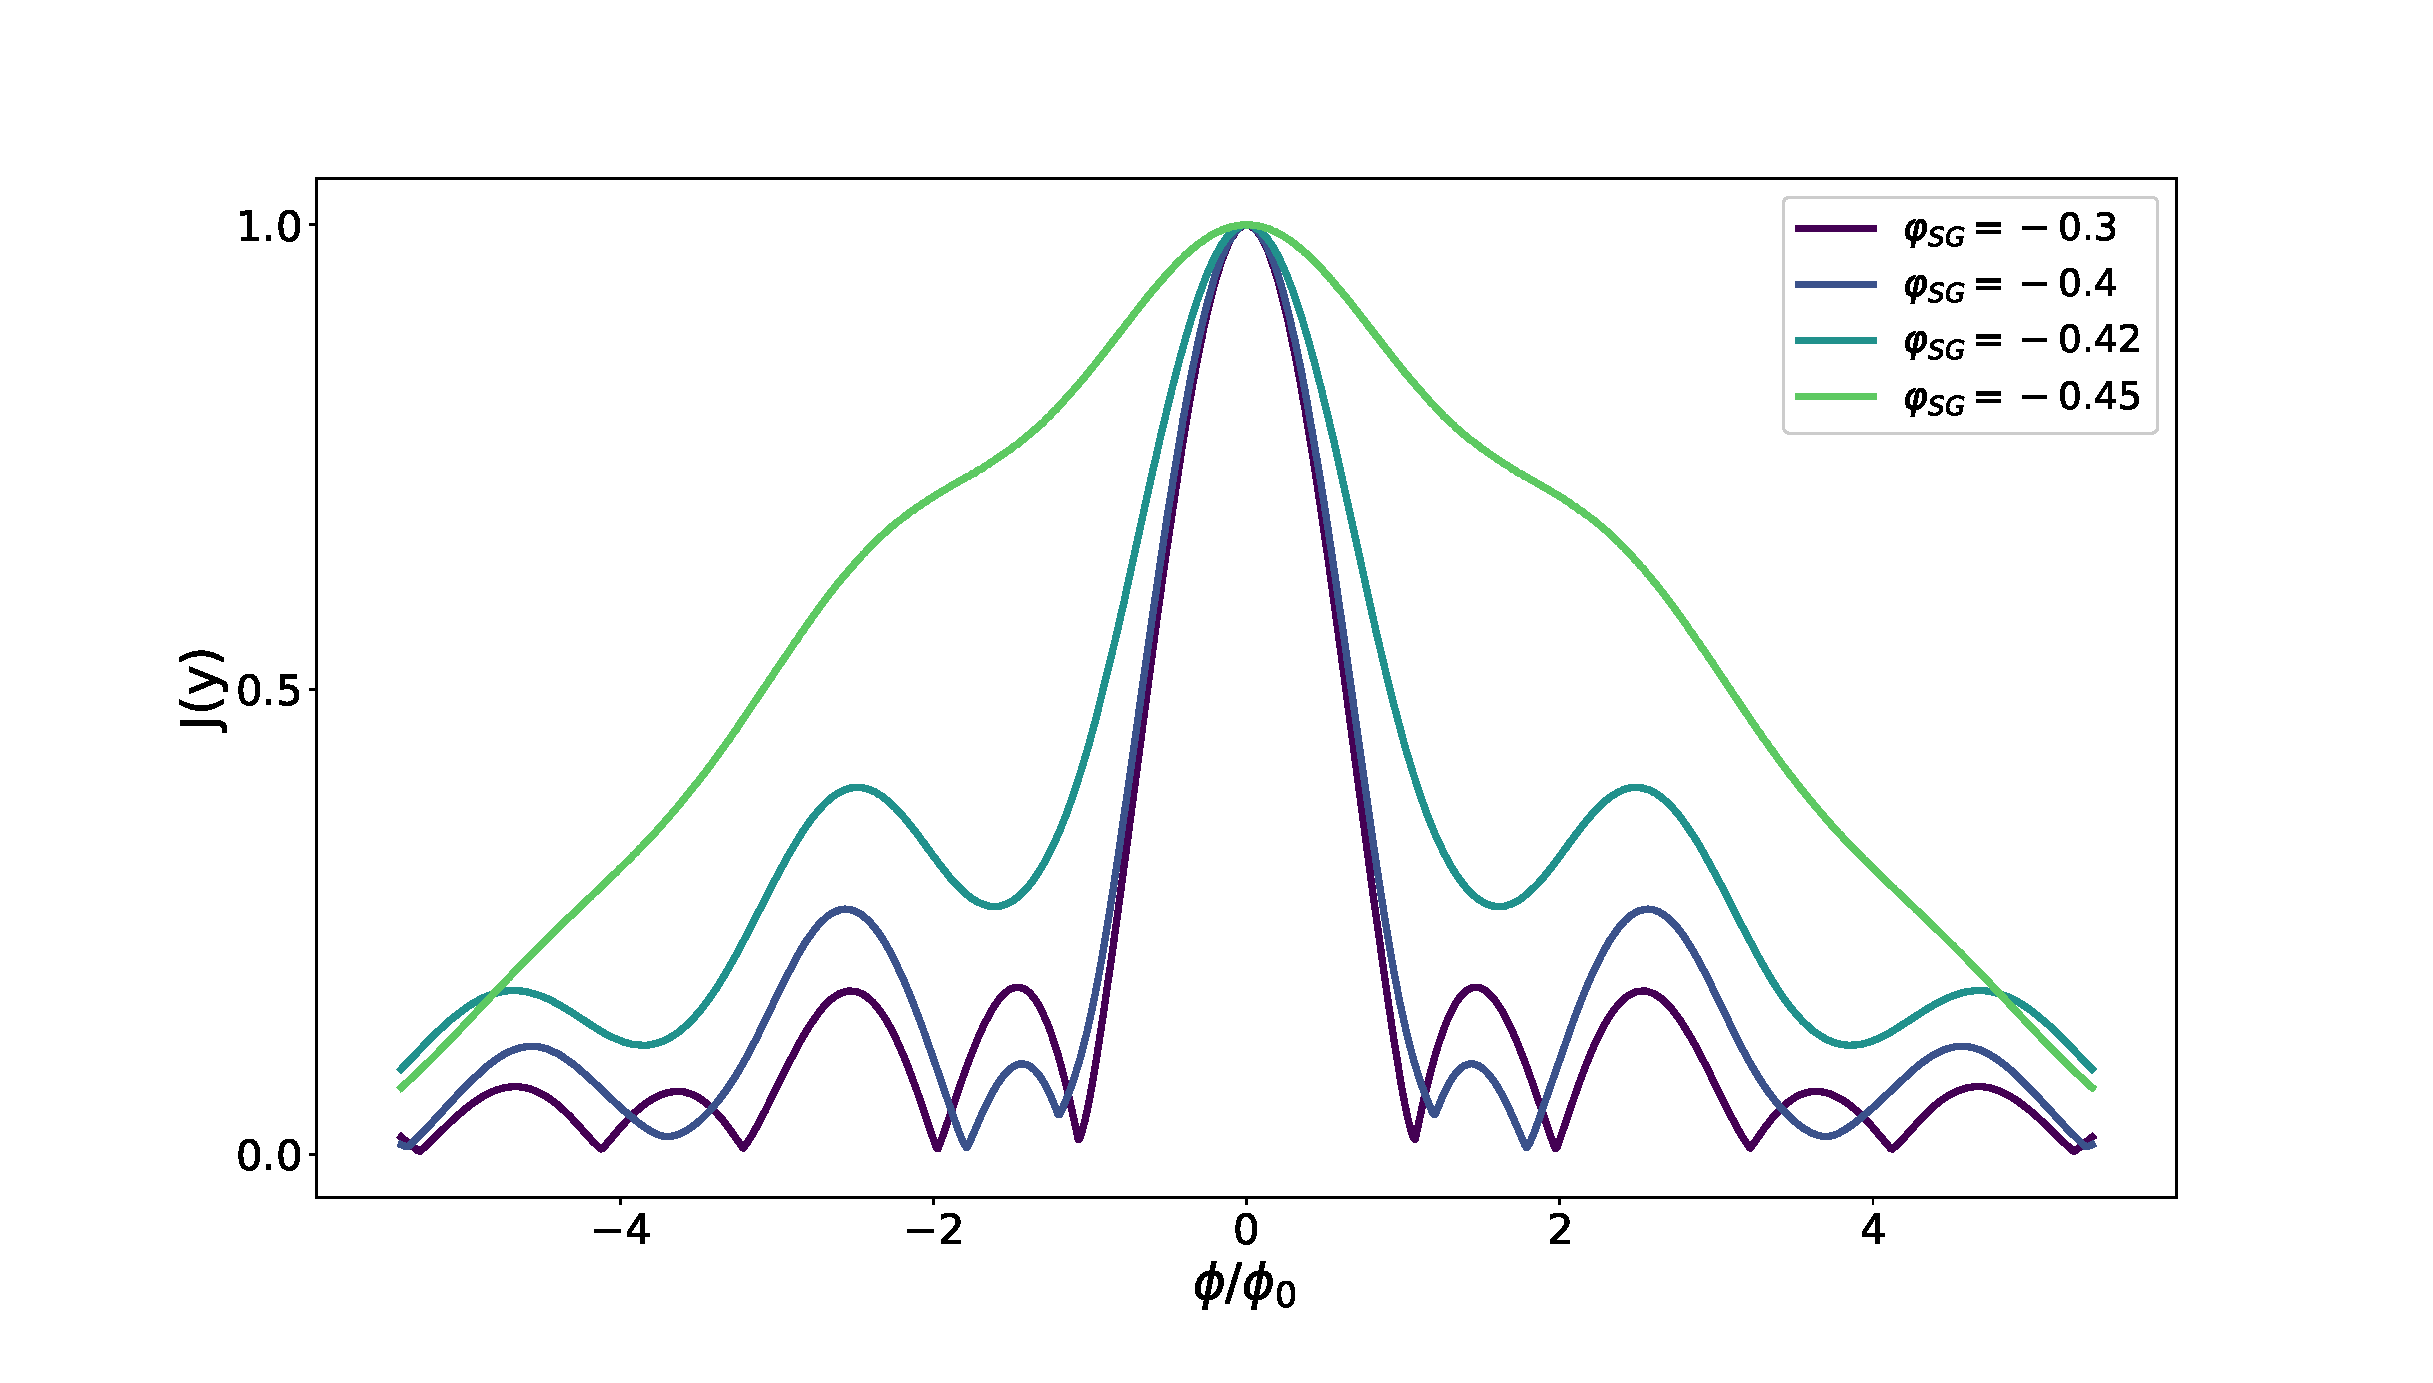
\includegraphics[width=\textwidth]{figure/numericalmodel/waveguide-ic}
\caption{Critical current in the wave-guide set-up. Similarly to the results of the QPC set-up, a transition from a beating pattern to a bell-shaped pattern can be observed.} \label{fig:waveguide-ic}
\end{minipage}
%\hspace{0.5cm}
\begin{minipage}[b]{0.5\linewidth}
\centering
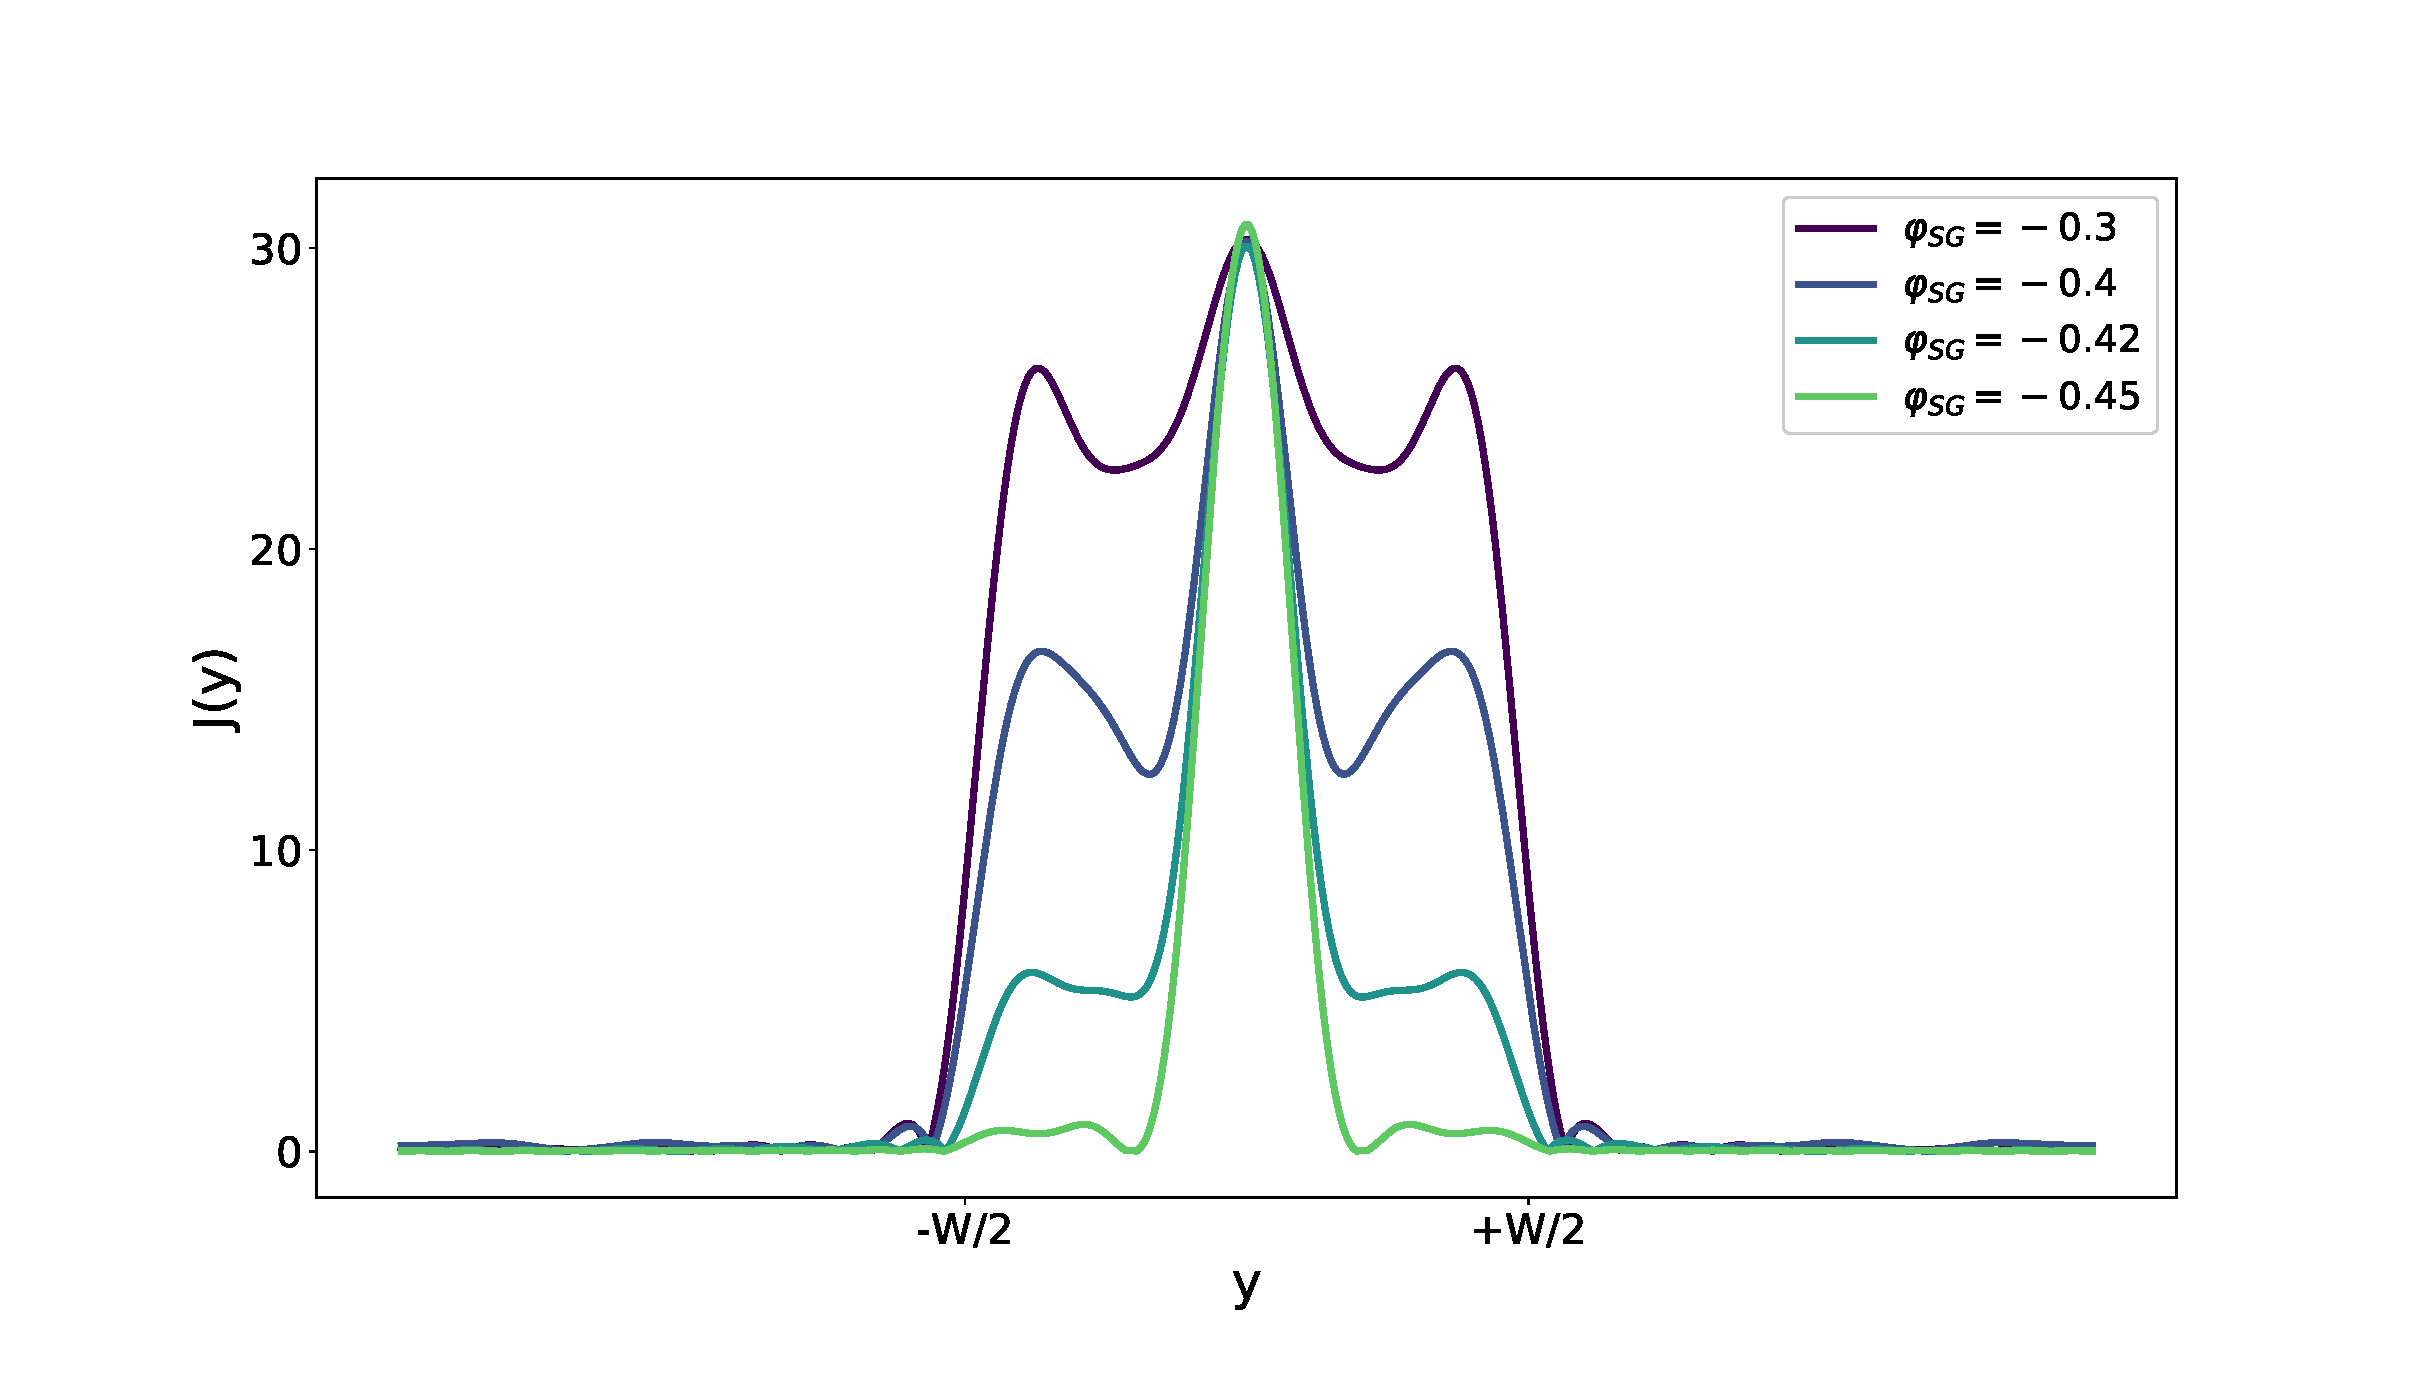
\includegraphics[width=\textwidth]{figure/numericalmodel/waveguide-jy}
\caption{Current density distribution along the y-axis of the wave-guide set-up. The curves can be found by fourier transforming the critical current from the plot on the left hand side.}\label{fig:waveguide-jy}
\end{minipage}
\end{figure}
The wave-guide set-up of figure \ref{fig:waveguide-system} is, again, a short and wide junction with a narrow channel. The current can be confined similarly to the QPC set-up. Because of the wide channel, the value for the high back-gate potential can be chosen to be relatively high. This is justifiable, since in comparison to the QPC set-up, the waveguide set-up is measured experimentally at higher charge carrier densities. The advantage of this set-up is the translation invariance in the x-direction because of its symmetry. This allows for fourier transformation of the current with the method of Dynes and Fulton \cite{Dynes1971}.

Figure \ref{fig:waveguide-ic} shows the normalized critical current. Similar to the results of the QPC simulation, a transition to a bell-shaped pattern can be observed. By fourier transforming the $I_c$-curves, the current density distribution along the width of the junction can be obtained. This current distribution is shown in figure \ref{fig:waveguide-jy}. For low values of the split-gate potential, the current density distribution is approximately rectangular. This implies that there is current flow below the top-gates. When the values of the split-gate potential become increasingly negative, the current density distribution resembles a sharp peak. In this situation, the current transport is confined to the the area not covered by the top-gate.

%Ergebnis: Strom wird eingeschränkt auf wenige Channels
\section{Summary Of This Chapter}
Results from simulations with \texttt{kwant} are presented. The experimental findings are matched very well. In the QPC and the wave-guide case, confinement of the critical current is demonstrated. 